
\documentclass[fleqn,addpoints]{exam}
\usepackage{amsmath}
\usepackage{graphicx}
\usepackage{float}
\usepackage{caption}
\usepackage{polynom}
\usepackage{mdwlist}

\newcommand{\degree}{\ensuremath{^\circ}} 

\printanswers

\ifprintanswers
\usepackage{2in1, lscape}
\fi

\title{Math 115 \\ Trigonometry Exam}
\date{June 21, 2011}

\author{}

\begin{document}

\maketitle  

\ifprintanswers
\else
\vspace{0.2in}
\makebox[\textwidth]{Name:\enspace\hrulefill}
\vspace{0.2in}

\begin{center}
\gradetable[h][pages]
% \bonusgradetable[h][pages]
\end{center}

\vspace{1 cm}

\fi

\section{Angles}
\begin{questions}

\question[3]
Convert $100 \degree$ to radians
\begin{solution}[4 cm]
\[
  100 \degree = 100 \degree \cdot \frac{\pi}{180\degree} = \frac{5 \pi}{9}
\]
\end{solution}

\question[3]
Convert $\dfrac{2 \pi}{5}$ from radians to degrees
\begin{solution}[4 cm]
\[
  \frac{2 \pi}{5} = \frac{2 \pi}{5} \cdot \frac{180 \degree}{\pi} = 72 \degree
\]
\end{solution}

\ifprintanswers
\else
\pagebreak
\fi

\section{Evaluation}

\question
\[
  \theta = \dfrac{7 \pi}{4}
\]

\begin{parts}
\part[1]
$\sin \theta = $
\begin{solution}[.75 cm]
$\sin \theta = - \dfrac{\sqrt{2}}{2}$
\end{solution}

\part[1]
$\cos \theta = $
\begin{solution}[.75 cm]
  $\cos \theta = \dfrac{\sqrt{2}}{2}$
\end{solution}

\part[1]
$\tan \theta = $
\begin{solution}[.75 cm]
  $\tan \theta = -1$
\end{solution}

\part[1]
$\csc \theta = $
\begin{solution}[.75 cm]
  $\csc \theta = - \sqrt{2}$
\end{solution}

\part[1]
$\sec \theta = $
\begin{solution}[.75 cm]
  $\sec \theta = \sqrt{2}$
\end{solution}

\part[1]
$\cot \theta = $
\begin{solution}[.75 cm]
  $\cot \theta = -1$
\end{solution}

\end{parts}

\question
\label{triangle3}
\begin{figure}[H]
  \centering
  \includegraphics[scale=.6]{triangle3.ps}
  \caption*{Question \ref{triangle3}}
\end{figure}

\begin{parts}
\part[1]
$\sin A = $
\begin{solution}[.75 cm]
  $\sin A = \dfrac{7}{11}$
\end{solution}

\part[1]
$\cos A = $
\begin{solution}[.75 cm]
  $\cos A = \dfrac{6 \sqrt{2}}{11}$
\end{solution}

\part[1]
$\tan A = $
\begin{solution}[.75 cm]
  $\tan A = \dfrac{7}{6}$
\end{solution}

\part[1]
$\csc A = $
\begin{solution}[.75 cm]
  $\csc A = \dfrac{11}{7}$
\end{solution}

\part[1]
$\sec A = $
\begin{solution}[.75 cm]
  $\sec A = \dfrac{11 \sqrt{2}}{12}$
\end{solution}

\part[1]
$\cot A = $
\begin{solution}[.75 cm]
  $\cot A = \dfrac{6 \sqrt{2}}{7}$
\end{solution}

\end{parts}
 
\question
$\cot \theta = -2$ and $\theta$ is in the second quadrant.

\begin{parts}

\part[1]
$\tan \theta = $
\begin{solution}[2 cm]
  $\tan \theta = - \dfrac{1}{2}$
\end{solution}

\part[3]
$\sin \theta = $
\begin{solution}[2 cm]
  $\sin \theta = \dfrac{\sqrt{5}}{5}$
\end{solution}

\part[3]
$\cos \theta = $
\begin{solution}[2 cm]
  $\sin \theta = - \dfrac{2 \sqrt{5}}{5}$
\end{solution}

\end{parts}

\vspace{1 cm}

\question[5]
\label{triangle2}
Solve for $x$

\begin{figure}[H]
  \centering
  \includegraphics[scale=.6]{triangle2.ps}
  \caption*{Question \ref{triangle2}}
\end{figure}

\begin{solution}[4 cm]
\begin{align*}
  \cos 60 \degree &= \frac{x}{12} \\
  \dfrac{1}{2} &= \frac{x}{12} \\
  x &= 6 \\
\end{align*}

\end{solution}


\ifprintanswers
\else
\pagebreak
\fi

\section{Graphing} 
 
\question
\label{graph}

$y = 2 \cos \left( \dfrac{x}{2} - \dfrac{\pi}{4} \right)$

\begin{parts}

\part[1] What is the amplitude?
\begin{solution}[2 cm] 
2
\end{solution}
 
\part[2] What is the period? 
\begin{solution}[2 cm]
$\dfrac{2 \pi}{1/2} = 4 \pi$
\end{solution}

\part[5] Draw the graph.  

\ifprintanswers
\else
\begin{figure}[H]
  \centering
  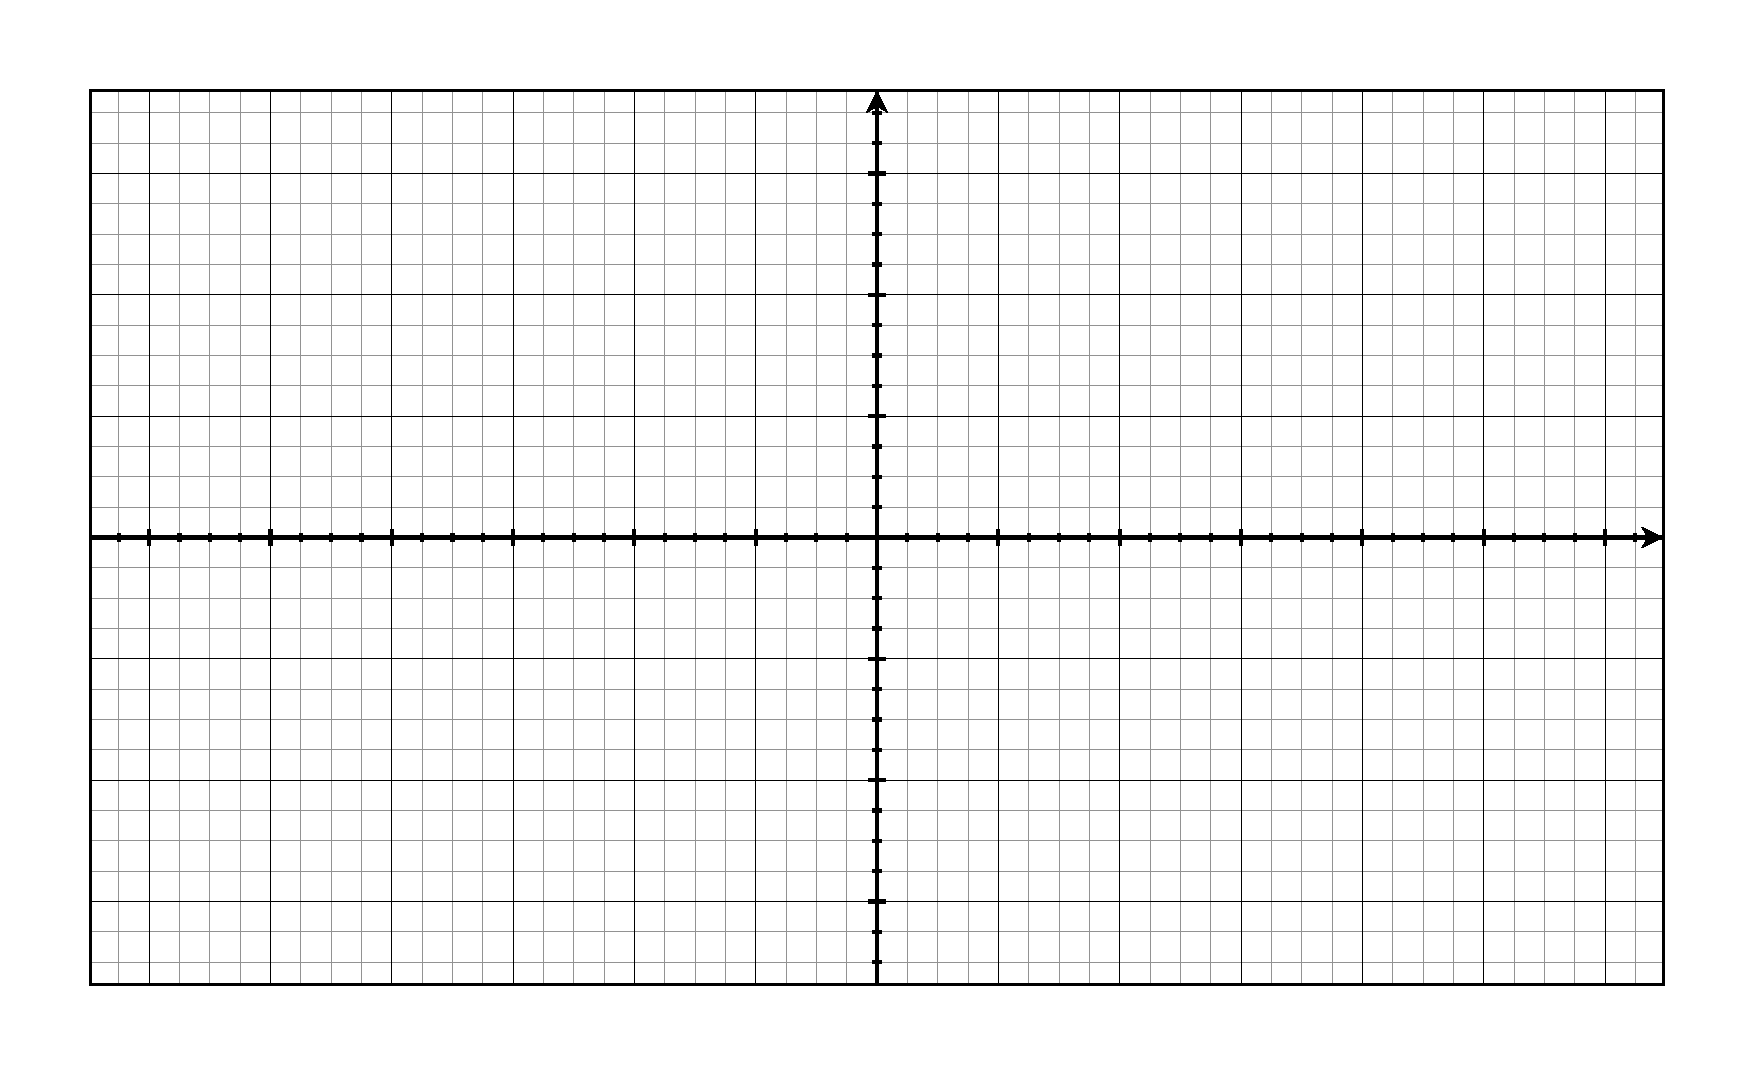
\includegraphics[scale=.6]{graph.eps}
  \caption*{Question \ref{graph}}
\end{figure}
\fi

\begin{solution}
\begin{figure}[H]
  \centering
  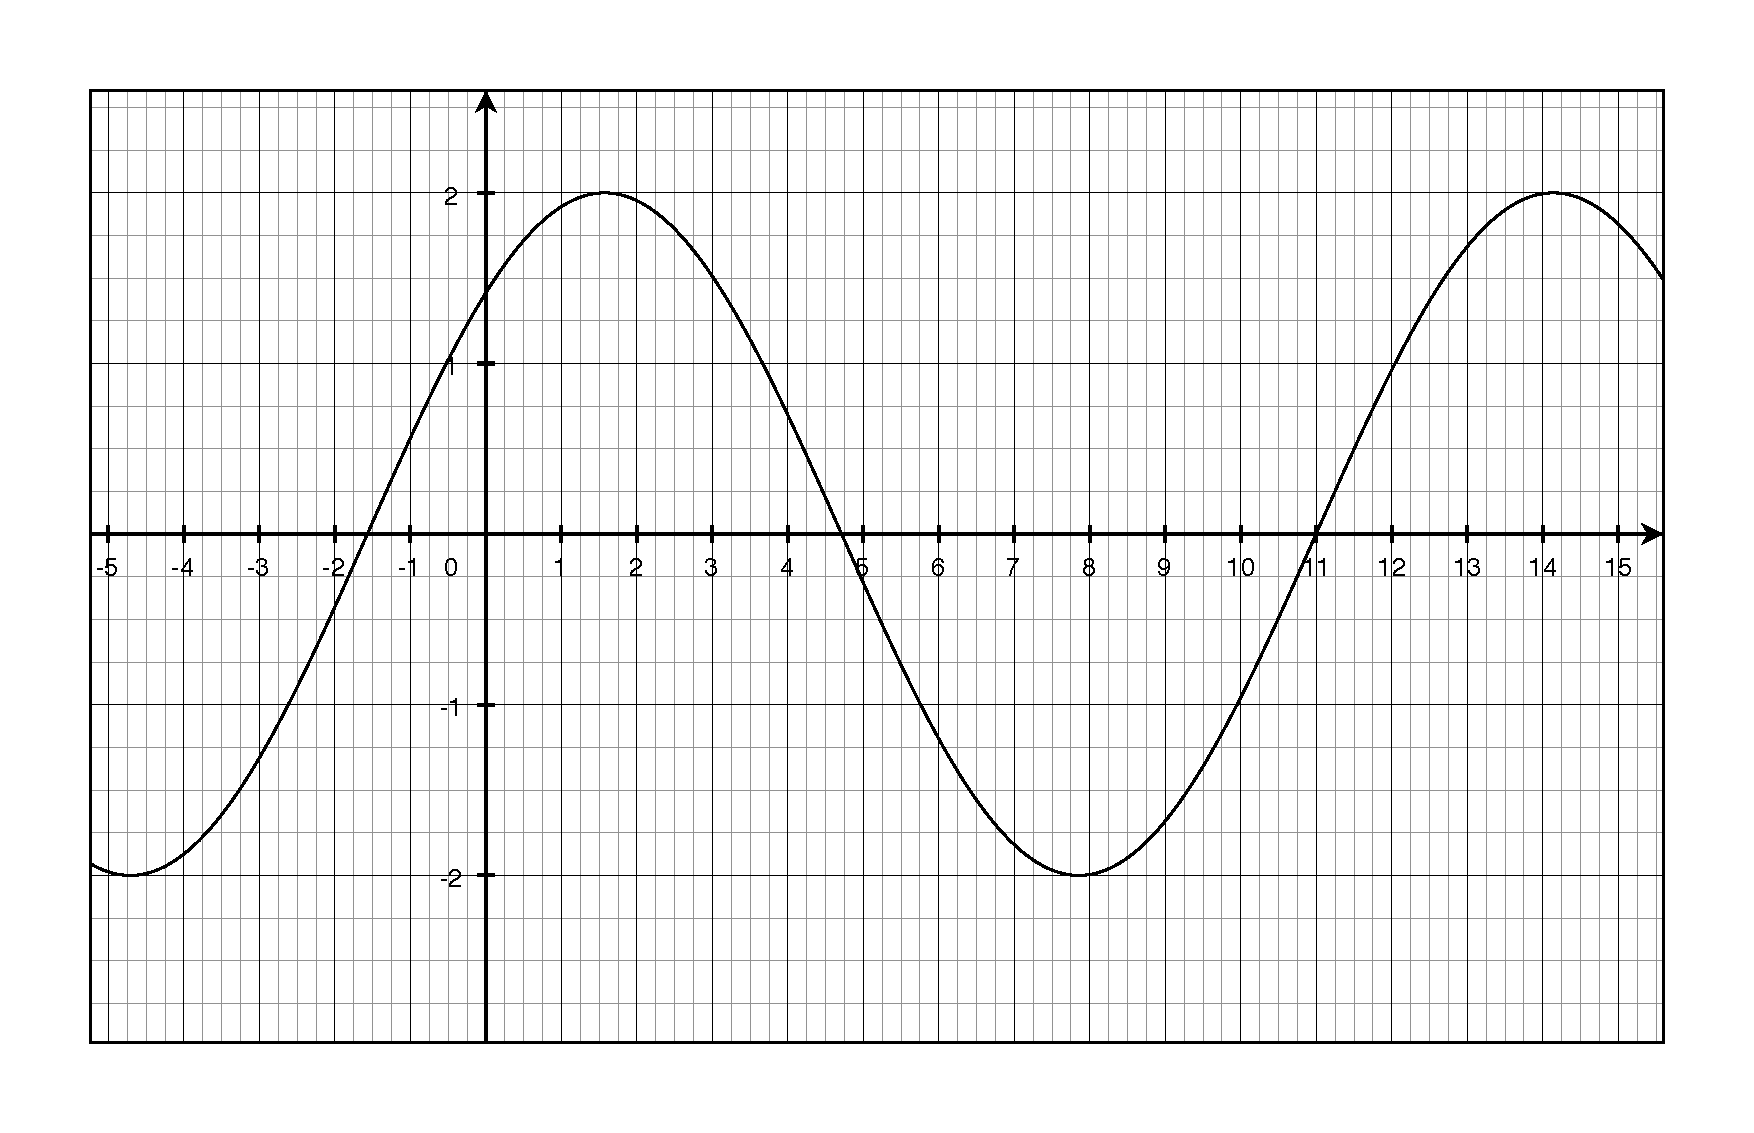
\includegraphics[scale=.3]{graph_solution.eps}
  \caption*{Question \ref{graph}}
\end{figure}
\end{solution}

\end{parts}

\ifprintanswers
\else
\pagebreak
\fi

\section{Inverse Trigonometric Functions} 

For questions \ref{inverse:first} to \ref{inverse:last}, evaluate the expression.

\question[2]
\label{inverse:first}
\[
  \arccos \frac{\sqrt{3}}{2} 
\]

\begin{solution}[1 cm]
  $\arccos \dfrac{\sqrt{3}}{2} = \dfrac{\pi}{6}$
\end{solution}

\question[3]
\[
  \arcsin \left( - \frac{\sqrt{2}}{2} \right)
\]
\begin{solution}[1 cm]
  $\arcsin \left( - \dfrac{\sqrt{2}}{2} \right) = - \dfrac{\pi}{4}$
\end{solution}

\question[5]
\label{inverse:last}
\[
  \cos \left( \arcsin \frac{5}{13} \right)
\]
\begin{solution}[2 cm]
  $\cos \left( \arcsin \dfrac{5}{13} \right) = \dfrac{12}{13}$
\end{solution}

\question[5]
\label{inverse:triangle}
Write $A$ as a function of $x$.

\begin{figure}[H]
  \centering
  \includegraphics[scale=.5]{triangle.ps}
  \caption*{Question \ref{inverse:triangle}}
\end{figure}

\begin{solution}[1 cm]
\begin{align*}
  \tan A &= \frac{x+1}{10} \\
  A &= \arctan \left( \frac{x+1}{10} \right)
\end{align*}

\end{solution}

 
\ifprintanswers
\else
\pagebreak
\fi

\section{Identities}

% \question[6]
% Simplify:

% \[
%   \frac{\sin x}{\csc x} + \frac{\cos x}{\sec x}
% \]

% \begin{solution}[3 cm]
% \end{solution}

For questions \ref{identity:first}--\ref{identity:last} verify the identity.

%% \question[5]
%% \label{identity:first}
%% \[
%%   2 \cos^2 x - 1 = 1 - 2 \sin^2 x
%% \]
%% \begin{solution}[3 cm]
%% \end{solution}

\question[5]
\label{identity:first}
\[
  \frac{1}{1 - \sin^2x} = 1 + \tan^2 x
\]
\begin{solution}[3 cm]
\[
  \frac{1}{1 - \sin^2x} = \frac{1}{cos^2 x} = \sec^2 x = 1 + \tan^2 x
\]

\end{solution}

\question[5]
\[
  \frac{1 - \cos x}{\sin x} = \frac{\sin x}{1 + \cos x}
\]
\begin{solution}[3 cm]
\begin{align*}
  \frac{1 - \cos x}{\sin x} &= \frac{1 - \cos x}{\sin x} \left( \frac{1 + \cos x}{1 + \cos x} \right) \\
  &= \frac{1 - \cos^2x}{\sin x (1 + \cos x)} \\
  &= \frac{\sin^2x}{\sin x (1 + \cos x) } \\
  &= \frac{\sin x}{1 + \cos x} \\
\end{align*}
\end{solution}

\question[5]
\[
  \sec^2x + \csc^2 x = \sec^2 x \csc^2 x 
\]
\begin{solution}[3 cm]
\begin{align*}
  \sec^2x + \csc^2 x &= \frac{1}{\cos^2 x} + \frac{1}{\sin^2 x} \\
  &= \frac{\sin^2 x + \cos^2 x}{\sin^2 x \cos^2 x} \\
  &= \frac{1}{\sin^2 x \cos^2 x} \\
  &= \sec^2 x \csc^2 x \\
\end{align*}
\end{solution}

\question[5]
\label{identity:last}
\[
  \frac{1 + \sec^2 x}{1 + \tan^2 x} = 1 + \cos^2 x
\]
\begin{solution}[3 cm]
\begin{align*}
  \frac{1 + \sec^2 x}{1 + \tan^2 x} &= \frac{1 + \sec^2 x}{\sec^2 x} \\
  &= \frac{1}{\sec^2 x} + \frac{\sec^2 x}{\sec^2 x} \\
  &= 1 + \cos^2 x \\
\end{align*}
\end{solution}

\section{Multiple Angle Formulas}

Find the exact value of
\question[5]
\[
  \sin 75 \degree  
\]
\begin{solution}[4 cm]
\begin{align*}
  \sin 75 \degree &= \sin(45 \degree + 30 \degree) \\
  &= \sin 45 \degree \cos 30 \degree + \cos 45 \degree \sin 30 \degree \\
  &= \frac{\sqrt{2}}{2} \cdot \frac{\sqrt{3}}{2} + \frac{\sqrt{2}}{2} \cdot \frac{1}{2} \\
  &= \frac{\sqrt{6} + \sqrt{2}}{4} \\
\end{align*}
\end{solution}

\question[5]
Write the product as a sum. 
\[
  \sin 2x \cos 3x
\]
\begin{solution}[4 cm]
\begin{align*}
  \sin 2x \cos 3x &= \frac{1}{2} \left[ \sin(2x + 3x) + \sin(2x - 3x) \right] \\
  &= \frac{1}{2} \left[ \sin(5x) + \sin(-x) \right] \\
  &= \frac{1}{2} \left[ \sin(5x) - \sin(x) \right] \\
\end{align*}
\end{solution}

\question[7]
Verify the identity:
\[
  \sin(x+y) \sin(x-y) = \sin^2 x - \sin^2 y
\]
\begin{solution}[4 cm]
\begin{align*}
  \sin(x+y) & \sin(x-y) = ( \sin x \cos y + \cos x \sin y)( \sin x \cos y - \cos x \sin y ) \\
  &= \sin^2 x \cos^2 y - \cos^2 x \sin^2 y \\
  &= \sin^2 x (1 - \sin^2 y) - (1 - \sin^2 x) \sin^2 y \\
  &= \sin^2 x - \sin^2 x \sin^2 y - (\sin^2 y - \sin^2 x \sin^2 y ) \\
  &= \sin^2 x - \sin^2 x \sin^2 y - \sin^2 y + \sin^2 x \sin^2 y \\
  &= \sin^2 x - \sin^2 y \\
\end{align*}
\end{solution}

% \question[5]
% Verify the identity:
% \[
%   \frac{\sin 4x}{\sin x} = 4 \cos x \cos 2x
% \]
% \begin{solution}[4 cm]
% \end{solution}

\ifprintanswers
\else
\pagebreak
\fi

\section{Laws of Sines and Cosines}

\question[5]
$A = 120 \degree$, $a = 3$, $b = \sqrt{3}$.  Find angle $B$.
\begin{solution}[4 cm]
$\sin 120 \degree = \sin 60 \degree = \dfrac{\sqrt{3}}{2}$

\begin{align*}
  \frac{\sin B}{\sqrt 3} &= \frac{\sin 120 \degree}{3} \\
  \frac{\sin B}{\sqrt 3} &= \frac{\sqrt{3}}{6} \\
  \sin B &= \frac{3}{6} \\
  \sin B &= \frac{1}{2} \\
  B &= 30 \degree \\  
\end{align*}

\end{solution}

\question[5]
$a = 4$, $b = 5$, $C = 60 \degree$.  Find the length of side $c$. 
\begin{solution}[4 cm]

$\cos 60 \degree = \dfrac{1}{2}$

\begin{align*}
  c^2 &= 4^2 - 5^2 - 2 \cdot 4 \cdot 5 \cdot \frac{1}{2} \\
  c^2 &= 21 \\
  c &= \sqrt{21} \\
\end{align*}
\end{solution}

\section{Extra Credit}
\bonusquestion[10]

Verify the identity:
\[
  \sin(a+b+c) + \sin a \sin b \sin c = \sin a \cos b \cos c + \sin b \cos a \cos c + \sin c \cos a \cos b  
\]

\begin{solution}[5 cm]
\begin{align*}
 \sin(a &+ b+c) + \sin a \sin b \sin c = \sin((a+b)+c) + \sin a \sin b \sin c \\
 &= \sin(a+b)\cos c + \cos(a+b)\sin c  + \sin a \sin b \sin c \\
 &= (\sin a \cos b + \cos a \sin b) \cos c + (\cos a \cos b - \sin a \sin b) \sin c \\
 &+ \sin a \sin b \sin c \\
 &= \sin a \cos b \cos c + \cos a \sin b \cos c + \cos a \cos b \sin c \\
 &- \sin a \sin b \sin c + \sin a \sin b \sin c \\
 &= \sin a \cos b \cos c + \sin b \cos a \cos c + \sin c \cos a \cos b \\
\end{align*}
\end{solution}

\end{questions}

\end{document}
